We have carried out a series of twenty forced-dissipative simulations of the SW
equations in a quadratic domain with periodic boundary conditions using the
standard open-source pseudo-spectral code FluidSim \cite[]{fluiddyn, fluidfft,
fluidsim}.
%
The simulations were started from zero initial
conditions and were run till a statistically stationary state was reached. The
equations were reformulated in terms of the three eigenmodes of the linearized
equations in Fourier space. One of these eigenmodes is zero for an irrotational
flow. We first carried out a few test simulations in which all three eigenmodes
were allowed to evolve in time. However, when only the two wave modes are
forced vorticity remains very small throughout the simulations and does not
affect the wave dynamics. Therefore, we chose to solve the equations only for
the two wave modes. As discussed in the previous section, a linear viscous term
in (\ref{eq_uu}) will not conserve momentum exactly and does not give a
strictly positive definite expression for energy dissipation. We have relaxed
the requirements of exact momentum conservation and positive definite energy
dissipation. Instead of using the nonlinear form of the viscous term in
(\ref{eq_uu}) we have used a higher order linear operator $ \nu_8 \nabla^{8} $
both in (\ref{eq_uu}) and (\ref{eq_h}), where $ \nu_8 $ is a `hyperdiffusion'
or a `hyperviscosity'. There is no strong physical motivation for this
modification but, as discussed by \cite{FargeSadourny1989}, a molecular viscous
operator of the form $\nu \nabla^2 $ is not necessarily a relevant model of the
actual small-scale dissipation for SW flows, which should rather be described
as a transition from two-dimensional to three-dimensional motions before
reaching the scales where dissipation actually occurs.
%
Time advancement is carried out by a classical fourth-order Runge-Kutta scheme
for the nonlinear term and an exact integration for the linear and dissipative
terms. This explicit integration is especially useful at very high resolution
and very large $c$ when the shortest waves are very fast. We use an adaptable
time step method which maximizes the time step over a standard
Courant-Friedrichs-Lewy condition \cite[]{Lundbladh1999,
AugierChomazBillant2012}.
%
Most of the aliasing is removed by truncating 8/9 of the modes along each
direction \cite[for a detail discussion on the issues of the non-conservation
of the non-quadratic energy and the aliasing errors in the truncated one-layer
shallow water model, see][]{FargeSadourny1989}. The resolution is characterized
by the number of nodes, $n$, in each direction and has been varied from 960
to 7680.
%
The wave speed $c$ has been varied over almost two orders of magnitude from 10
to 700. The wave modes are forced in a shell in spectral space corresponding to
relatively small wave numbers, $ 5 \delta k < |\kk| < 8 \delta k$, where $
\delta k = 2 \pi /L $ and $ L $ is the length of the side of the quadratic
domain. The forcing is white noise in time and designed so that the energy
injection rate is normalized to unity at each time step. The energy is
dissipated at the smallest resolved scales by hyperviscosity. The value of the
hyperviscosity, $\nu_8$, is chosen in such a way that the maximum wave number
is larger than the dissipation wave number
\begin{equation}
k_{d} = \left( \frac{{\nu_8}^3}{\eps} \right)^{-\frac{1}{22}},
\end{equation}
where $ \eps $ is the mean energy dissipation rate. We found that $ k_{d}
\simeq \kmax/ 2.5$, where $\kmax = (8/9)\pi n/L $ is the maximum wave number,
is sufficient in order for dissipation spectra to be resolved. Since the energy
injection rate is normalized to unity and all simulations reach a stationary
state in which dissipation is equal to the injection rate, $ \nu_8 $ can be
chosen already from the start so that this condition will be fulfilled in the
stationary state. The strength of the stratification is characterized by a
Froude number, defined as
\begin{equation} \label{Fr}
F_f = \frac{\varepsilon^{1/3}}{c k_f^{1/3}} \, ,
\end{equation}
a parameter that can be determined from the start of each simulations.
The  simulation parameters are listed in table 1.


\begin{table}
\begin{center}

\label{Table1}
\begin{tabular}{lrrrrrrrr}

\toprule
{} &   $n$ &  $c$ &  $\nu_8$ &  $\eps$ &  $ k_{d}  / {k_f} $ &   $F_f$ &    $t_{\max}$ \\
\midrule
W1  &   960 &   10 & 1.56e-10 &        1.04 &                    28.8 &   0.111 &                49.9 \\
W2  &  1920 &   10 & 9.68e-13 &        1.06 &                    57.7 &   0.112 &               49.8 \\
W3  &  3840 &   10 &    6e-15 &         1.10&                     115 &   0.113 &               49.9 \\
W4  &  7680 &   10 & 3.72e-17 &        1.18 &                     231 &   0.116 &               49.9 \\
W5  &   960 &   20 & 1.56e-10 &           1.00 &                    28.8 &   0.055 &              49.9 \\
W6  &  1920 &   20 & 9.69e-13 &        1.02 &                    57.7 &  0.0553 &                120 \\
W7  &  3840 &   20 & 6.01e-15 &        1.08 &                     115 &  0.0563 &                120 \\
W8  &  7680 &   20 & 3.72e-17 &        1.21 &                     231 &  0.0585 &                 120 \\
W9  &   960 &   40 & 1.56e-10 &          1.00 &                    28.8 &  0.0274 &                49.8 \\
W10 &  1920 &   40 & 9.68e-13 &       1.00 &                    57.7 &  0.0274 &               49.8 \\
W11 &  3840 &   40 &    6e-15 &        1.06 &                     115 &   0.028 &               49.8 \\
W12 &   960 &  100 & 1.56e-10 &       1.00 &                    28.8 &   0.011 &                49.8 \\
W13 &  1920 &  100 & 9.69e-13 &        1.01 &                    57.7 &   0.011 &                 120 \\
W14 &  3840 &  100 & 6.01e-15 &        1.06 &                     115 &  0.0112 &                 120 \\
W15 &  7680 &  100 & 3.72e-17 &        1.22 &                     231 &  0.0117 &                95.8 \\
W16 &   960 &  400 & 1.56e-10 &        1.14 &                    28.8 & 0.00287 &                 120 \\
W17 &  1920 &  400 & 9.69e-13 &        1.15 &                    57.7 & 0.00288 &                 120 \\
W18 &  3840 &  400 & 6.01e-15 &        1.12 &                     115 & 0.00286 &                119 \\
W19 &   960 &  700 & 1.56e-10 &        1.27 &                    28.8 &  0.0017 &                49.8 \\
W20 &  1920 &  700 & 9.68e-13 &        1.05 &                    57.7 &  0.0016 &                49.8 \\
\bottomrule

\end{tabular}
\caption{Parameters for all simulations. $ n $: number of nodes in each
direction, $ c $: wave speed, $ \nu_8 $: hyperviscosity, $ \eps $: time
averaged mean energy dissipation in the stationary state, $ k_{d}/ k_f $: ratio
between dissipation wave number and forcing wave number, $ F_f $: Froude
number, $ t_{max} $: end time of simulation.}
\end{center}
\end{table}





\begin{figure}
\centerline{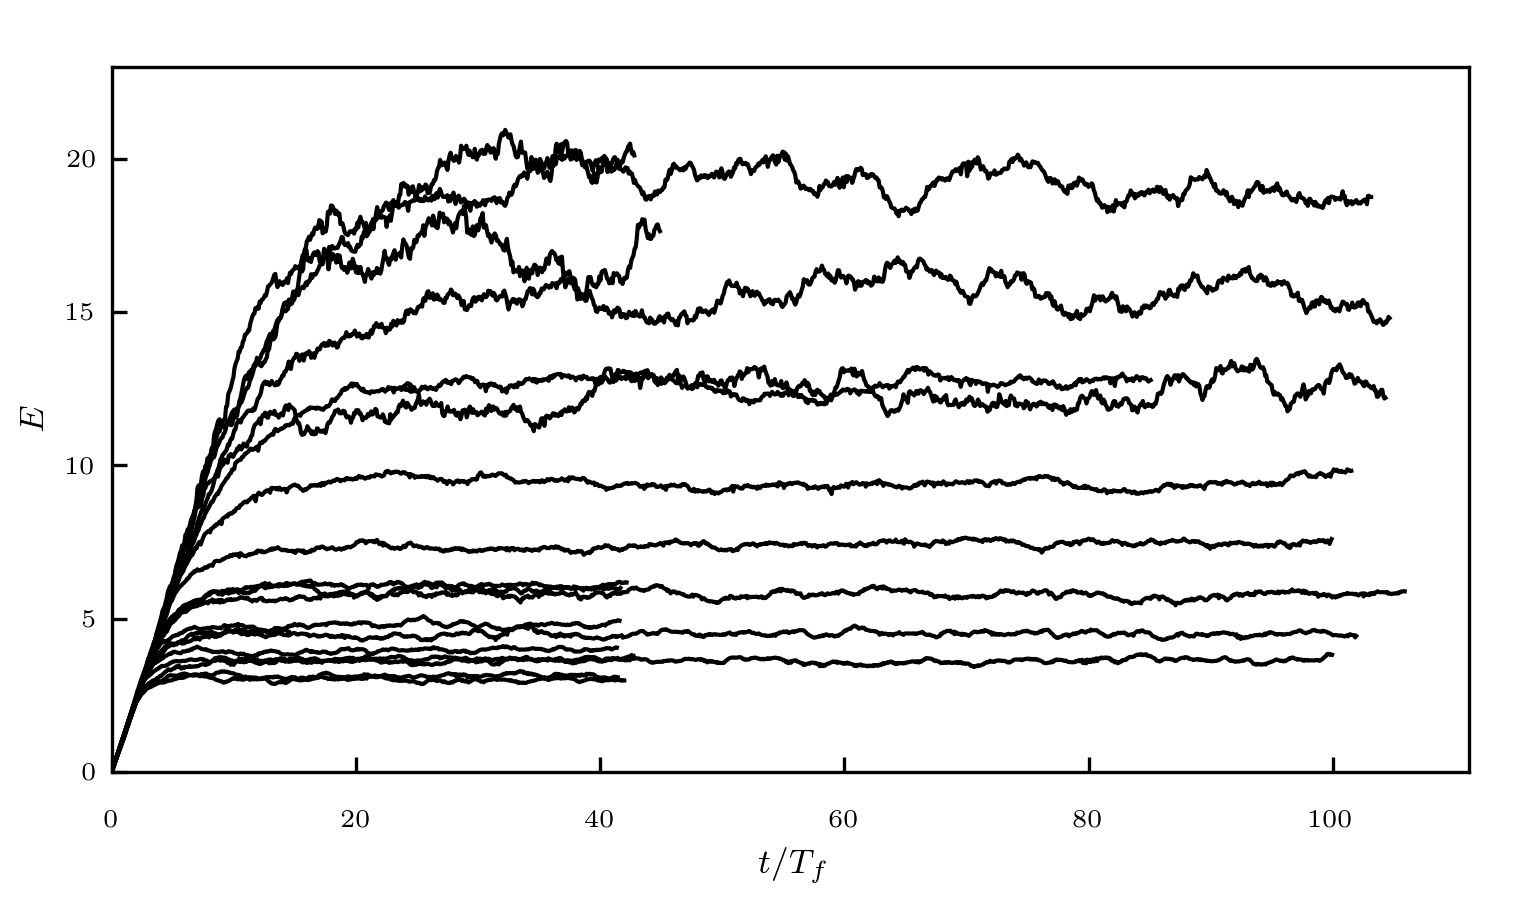
\includegraphics[width=5.12in]{../Pyfig/fig_Emean_time}}
\caption{Space averaged energy, $E = E_K + E_A $, versus time for all
simulations. }
\label{fig_Evstime}
\end{figure}

\begin{figure}
\centerline{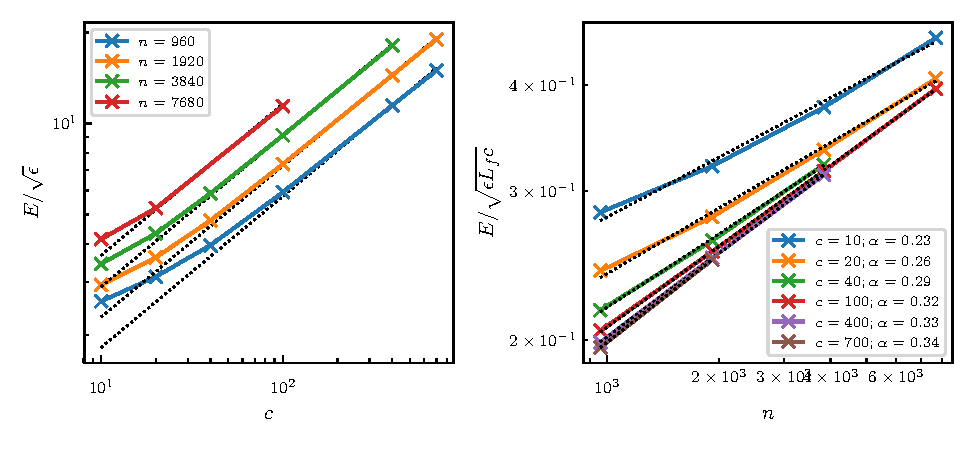
\includegraphics[width=5.8in]{../Pyfig/fig_energy_w}}
\caption{Left: Mean energy in the stationary state versus $ c $ for different
resolutions. The lines have slope $ 0.5 $, corresponding to $ E \propto c^{1/2}
$. Right: Normalized mean energy in the stationary state versus resolution $ n
$ for different $ c $.}
\label{MeanE}
\end{figure}



The time evolution of mean energy is shown in figure~\ref{fig_Evstime} for all
twenty simulations. After an initial period of growth, mean energy is leveling
out at different values for different runs. This is not the same picture as we
see in simulations of three-dimensional incompressible turbulence or stratified
turbulence, where all curves would have leveled out more or less at the same
value. We find that mean energy in the stationary state is a function of both $
c $ (or the Froude number) and resolution $ n $ and that the functional
dependence can be approximately written as
\begin{equation} \label{MeanEnergy}
E \propto \sqrt{L_f c \eps} \, n^{\alpha}  \, ,
\end{equation}
where $ L_f = \pi/k_f $ is the forcing scale. In figure~\ref{MeanE} to the
left, we see $ E/\sqrt{\eps} $ as function of $ c $ for different resolutions $
n $. For each resolution the points are approaching a power law $ C_n c^{1/2} $
with increasing values of $ C_n $ for increasing $ n $. In the same figure to
the right we see $ E/\sqrt{L_f c \eps} $ for different values of $ c $. For
each $ c $ the points follow a power law $ n^{\alpha} $, where $ \alpha $ is
becoming slightly larger with increasing $ c $, approaching almost the same
value $ \alpha \approx 0.33 $ for the three highest values of $ c $. The
relation (\ref{MeanEnergy}) can be reformulated as
\begin{equation} \label{Dissipation}
\frac{\eps} {(E^{3/2} / L_f)} \propto \frac{E^{1/2}}{c} n^{-2\alpha}
\end{equation}
Since the simulations are well resolved the dependence on resolution should not
be interpreted as consequence of the numerics but rather as a Reynolds number
effect, although it is not hundred percent clear how a Reynolds number should
be defined in our case. We may note, however, that $ n $ is proportional $
k_{d} / k_f $ and the corresponding ratio in Kolmogorov turbulence scales as $
Re^{3/4} $ since the Kolmogorov scale is proportional to $ \nu^{3/4} $, where $
\nu $ is the kinematic viscosity. If we simply define a Reynolds number as
\begin{equation}
Re = \left ( \frac{k_d} {k_f} \right )^{4/3} \, ,
\end{equation}
we can substitute $ n^{-2\alpha} $ in (\ref{Dissipation}) with $ Re^{-8
\alpha/3} $. The normalised energy dissipation on the left hand side of
(\ref{Dissipation}) will thus go to zero in the limit of large Reynolds number.
This is very different from three-dimensional turbulence where there is a local
Richardson-Kolmogorov cascade, in which energy is successively transfered from
large to small scales of motion. That the cascade is local means that eddies of
a particular scale are not directly influenced by eddies of widely different
scales. As a consequence, the normalized dissipation is of the order of unity
independent of Reynolds number \cite[]{Pope, TennekesLumley}. A review of the
experimental evidence and theoretical implications of this fundamental law of
Kolmogorov turbulence is given by \cite{Vassilicos2015}. Our result
(\ref{Dissipation}) suggests that SW wave turbulence does not fit into the
paradigm of a local Richardson-Kolmogorov cascade. Moreover, it is not only in
the limit of large Reynolds number the normalized dissipation will go to zero
but also in the limit of strong stratification, $ E^{1/2}/c \rightarrow 0 $.
This is different from three-dimensional stratified turbulence where the ratio
on the left hand side of (\ref{Dissipation}) is of the order of unity in the
limit of strong stratification \cite[]{Lindborg2006, Brethouwer2007}.


The `four-fifths law' for the third order structure function of Kolmogorov
turbulence is often derived using the assumption of a local cascade
\cite[]{Vassilicos2015} or the assumption that dissipation stays finite in the
limit of large Reynolds number \cite[]{Frisch}. As we just discussed, these
assumptions seem to be violated in the case of SW wave turbulence.
Nevertheless, the analogous law (\ref{eq_Kolmo}) that we derived for SW wave
turbulence is satisfied with a high degree of accuracy in our simulations. In
figure~\ref{Flux} we see the spectral energy flux from run W7 to the left and
the third order structure function to the right. There is a broad constant flux
range with equipartition between KE and APE flux and an almost equally broad
range where (\ref{eq_Kolmo}) is satisfied, with equipartition between the two
third order structure functions associated with KE and APE. The assumptions of
a local cascade and finite dissipation do not seem to be necessary in order for
the third order structure function law (\ref{eq_Kolmo}) to be valid.



\begin{figure}
\centerline{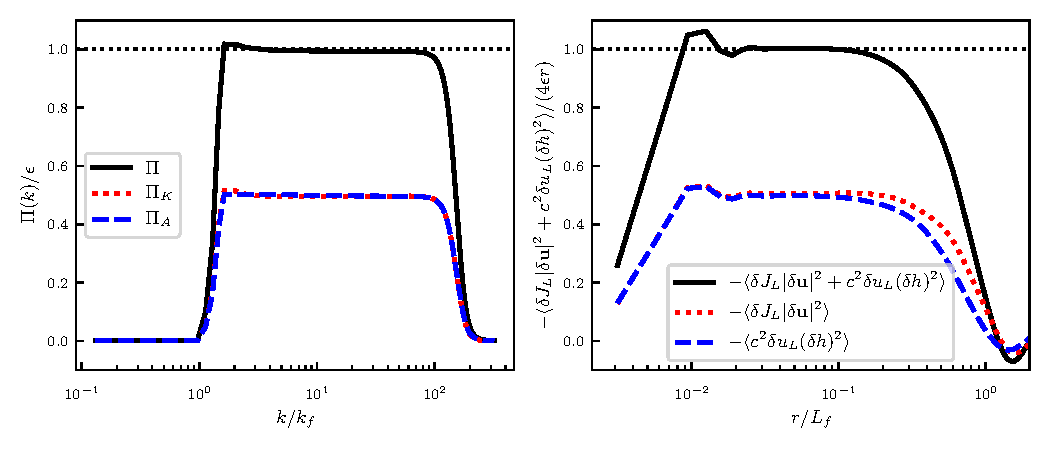
\includegraphics[width=5.8in]{../Pyfig/fig_flux_struct_combined}}
\caption{Left: Time averaged normalised spectral energy fluxes versus $ k/k_f
$. Right: Time averaged normalised third order structure functions versus $
r/L_f $. From run W7. }
\label{Flux}
\end{figure}


\begin{figure}
\centerline{\includegraphics[width=3.15in]{../Pyfig/fig_spatiotempspectra}}
\caption{Frequency spectra of KE and APE for different $ k = \mid {\bf k} \mid
$, from run W7. The spectra are plotted as functions of $\omega/\omega_l$,
where $\omega_l = c k$. From top to bottom: $ k /\delta k = 12$, 27, 62, 143,
327, and 746. }
\label{fig_spatiotemp_spectra}
\end{figure}

\begin{figure}
\centerline{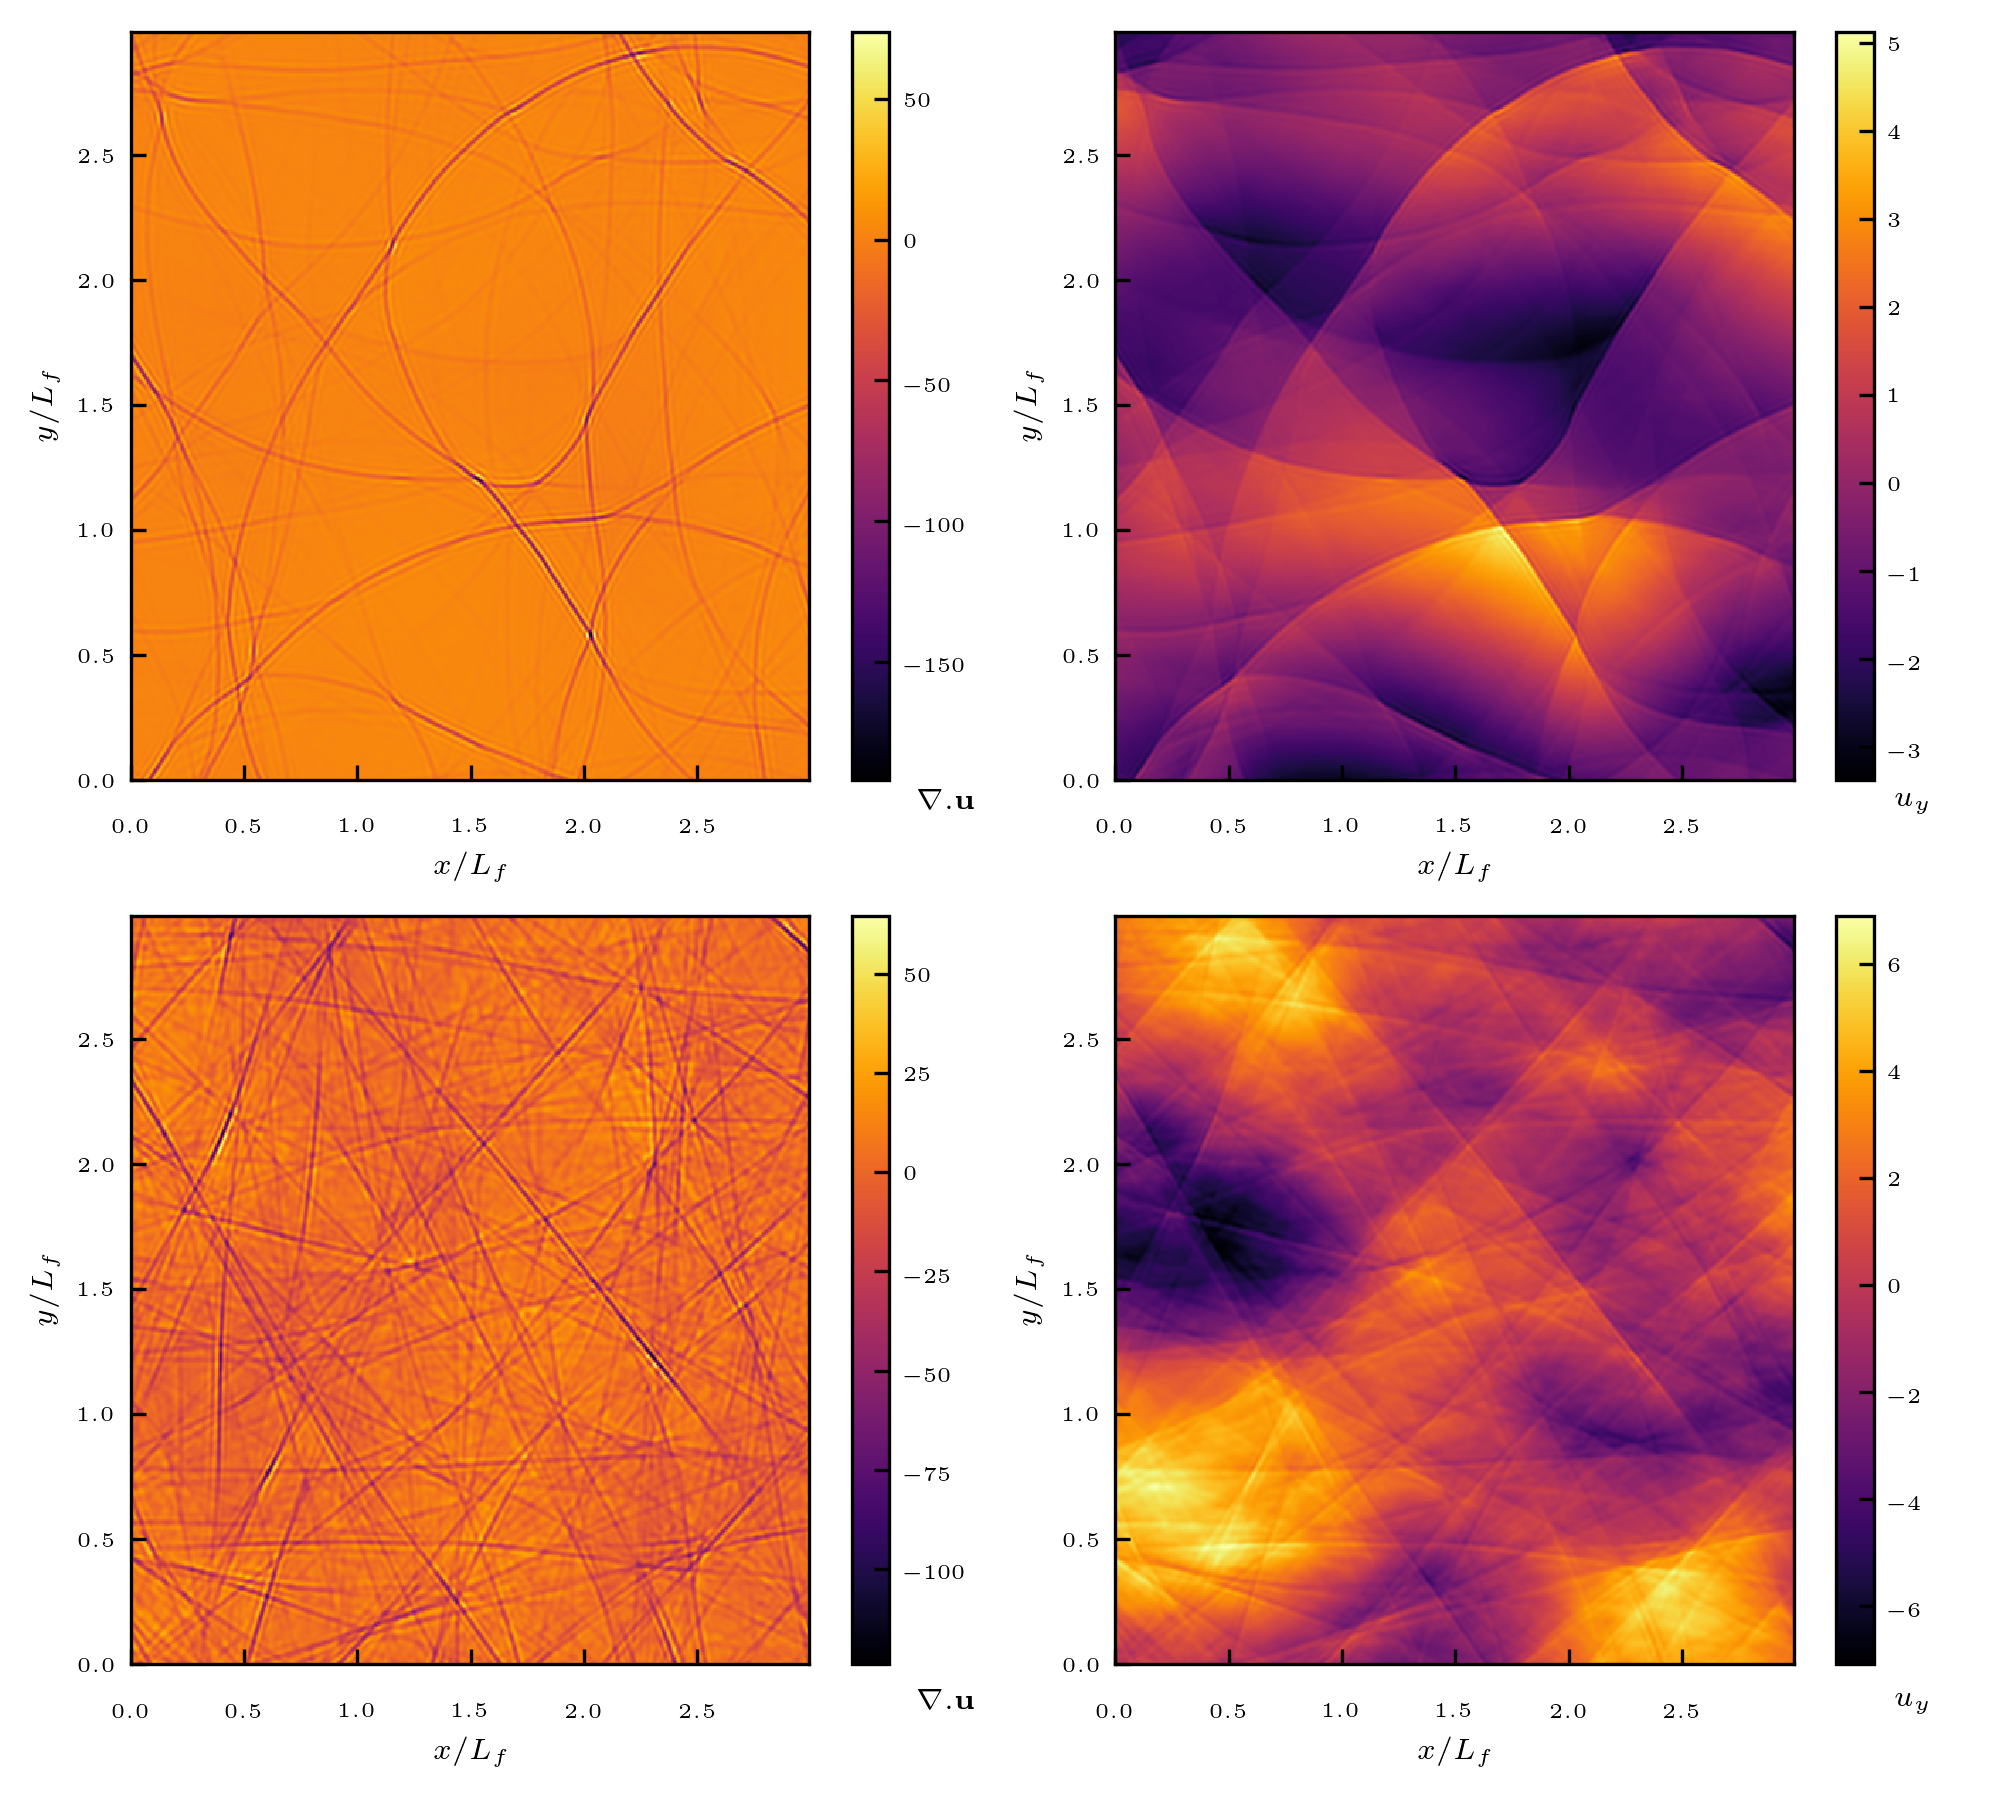
\includegraphics[width=6.0in]{../Pyfig/fig_phys_fields_wave}}
\caption{Left: divergence $ \bnabla \cdot {\bf u} $. Right: velocity component in the $ y $-direction: $ u_y $. Top: run W6. Bottom: run W17.  }
\label{Physical}
\end{figure}

\begin{figure}
\centerline{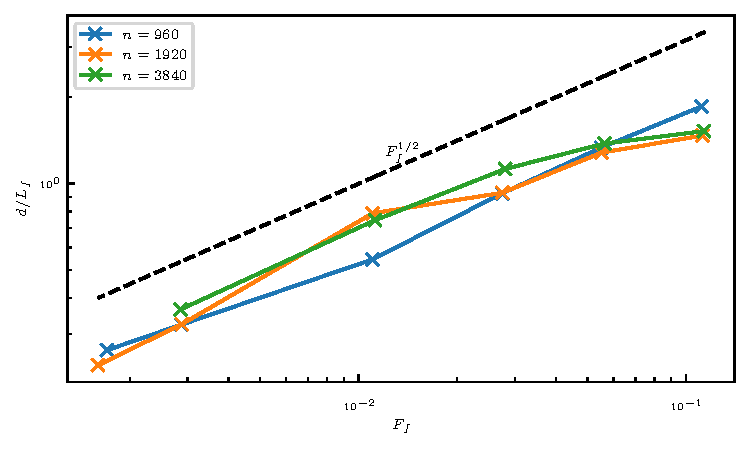
\includegraphics[width=8cm]{../Pyfig/fig_shock_sep.pdf}}
\caption{Mean distance between the shocks as function of Froude number.  }
\label{fig_distance}
\end{figure}




The equipartition of KE and APE spectral fluxes suggests that the flow to
leading order may be described as a collection of linear gravity waves with
equipartition of KE and APE in each mode. To investigate this further we have
collected time series of the flow variables from Fourier modes whose magnitude
fall within certain shells, $ \mid {\bf k} \mid \in [ k -\delta k/2, \; k+
\delta k/2] $, and computed temporal power law spectra from these time series
and averaged over all wave numbers in each shell. In other words we have
computed KE and APE frequency spectra corresponding to different magnitudes of
modes. Figure~\ref{fig_spatiotemp_spectra} presents such spectra plotted as a
functions of the normalized frequency $\omega/\omega_l$, where $ \omega_l = kc
$ is the linear wave frequency, The spectra are strongly dominated by peaks at
$\omega = \omega_l$. As can be seen, there is equipartition between KE and APE
in each shell. Although the widening of the peaks around the linear frequency
most likely is an effects of nonlinearities, we can quite safely conclude that
the time evolution of the flow variables in each Fourier mode to leading order
can be described as a linear wave.

Visualizations of the flow field give a completely different picture from what
may be expected from a collection of linear gravity waves. They are totally
dominated by the appearance of shock waves. In figure~\ref{Physical} we see
the divergence, $ \nabla \cdot {\bf u} $, to the left and the velocity
component in the $ y $-direction, $ u_y $, to the right. The two figures at the
top are from run W6 while the two figures at the bottom are from run W17. The
difference between the two runs is that $ c $ is larger by a factor of $ 20 $
in W17 as compared to W6. To the left we see the shocks displayed as elongated
bands of negative divergence. That the divergence is negative at the shocks can
be understood from the fact that the velocity component perpendicular to the
shock always has a negative jump in the direction of shock propagation.
Apparently, the mean distance between the shocks is considerably smaller in run
W17 with the larger value of $ c $ compared to run $ W6 $ with the smaller
value of $ c $. The shocks are also visible in the figures to right where $ u_y
$ is displayed. It may be interesting to note that the shocks along the $ x
$-axis appear as extra sharp in this plot, since there is a strong jump of $
u_{y} $ over these shocks, while the shocks along the $ y $-axis are hardly
visible, since there is no jump of $ u_{y} $ over these. In the two figures to
the right we see a variation of the flow field over the length scale $ L_f $
which is not seen in the two figures to the left. This variation is evidently a
footprint of the random forcing. Although the forcing length scale $ L_f $ is
the same in the two simulations the mean distance, $ d $, between the shocks is
much smaller in run $ W17 $ than in run $ W6 $, which may seem a little bit
surprising. We have calculated $ d $ by counting the number of negative spikes
of the divergence along ten lines parallel to the $ x $-axis and ten lines
parallel to the $ y $-axis and then divided total length of all the lines by
the number of spikes. Generally, we found that $ d \sim c^{-1/2} $, or
\begin{equation} \label{MeanDistance}
d \propto L_f F_f ^{1/2} \, ,
\end{equation}
independent of resolution $ n $. In figure~\ref{fig_distance} we have plotted
$ d/L_f $ versus Froude number for all twenty runs. As can be seen the points
follow the $ F_f^{1/2} $-curve quite well, although there seems to be a slight
systematic deviation at the highest $ F_f $, which may be due to the fact that
$ d $ is rather close to the length of the side of the box for the largest $
F_f $.

\begin{figure}
\centerline{
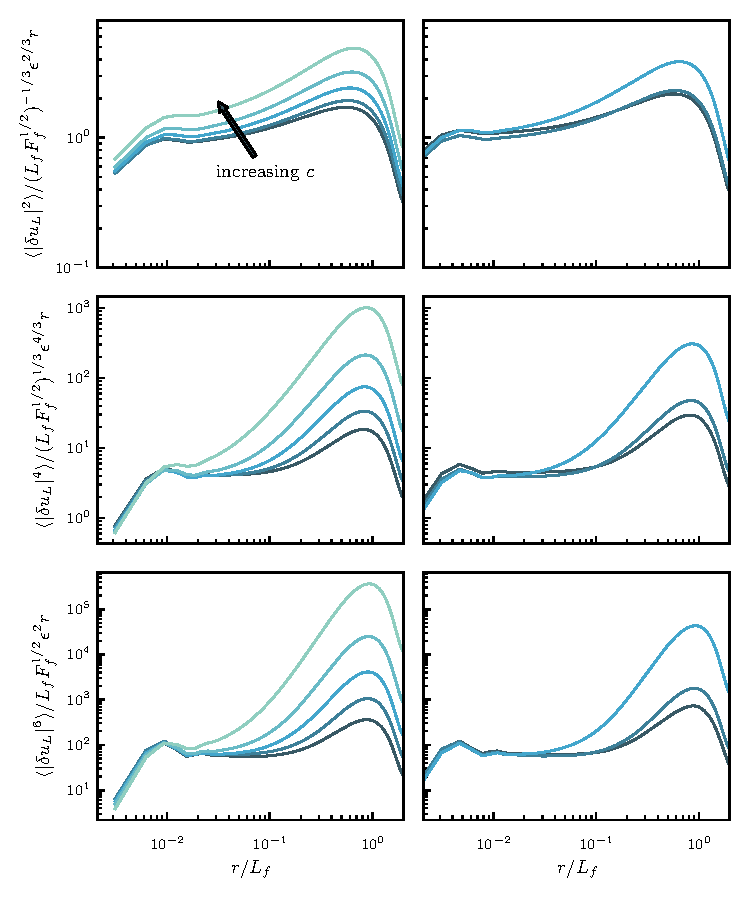
\includegraphics[width=5.0in]{../Pyfig/fig_struct_order_246}}
\caption{From top to bottom: second, fourth and sixth order compensated and
normalised longitudinal structure functions. Left: runs with $ n=3840 $: W3,
W7, W11 and W18. Right: runs with $ n = 7860 $: W4, W8 and W15. }
\label{fig_StrucFunc}
\end{figure}

\begin{figure}
\centerline{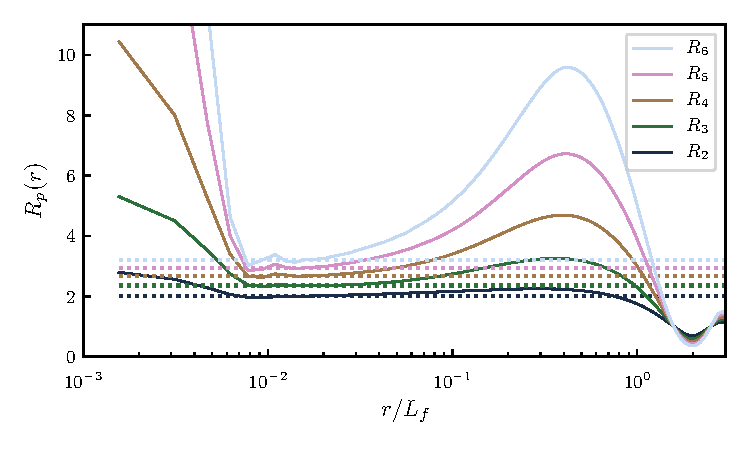
\includegraphics[width=8cm]{../Pyfig/fig_ratio_strfct}}
\caption{
Ratio of the structure functions
$R_p(r) = \mean{|\delta u_L|^p} / \mean{|\delta u_T|^p}$ from run W4,
for $ p = 2, \, 3, \, 4, \, 5, \, 6. $
The dotted straight lines indicate the values predicted by (\ref{Ratio}):
$R_2 = 2$, $R_3 = 3\pi/4$,  $R_4 = 8/3$, $ R_5 = 15 \pi /16 $ and $ R_6 = 16/5 $.}
\label{fig_ratio}
\end{figure}

\begin{figure}
\centerline{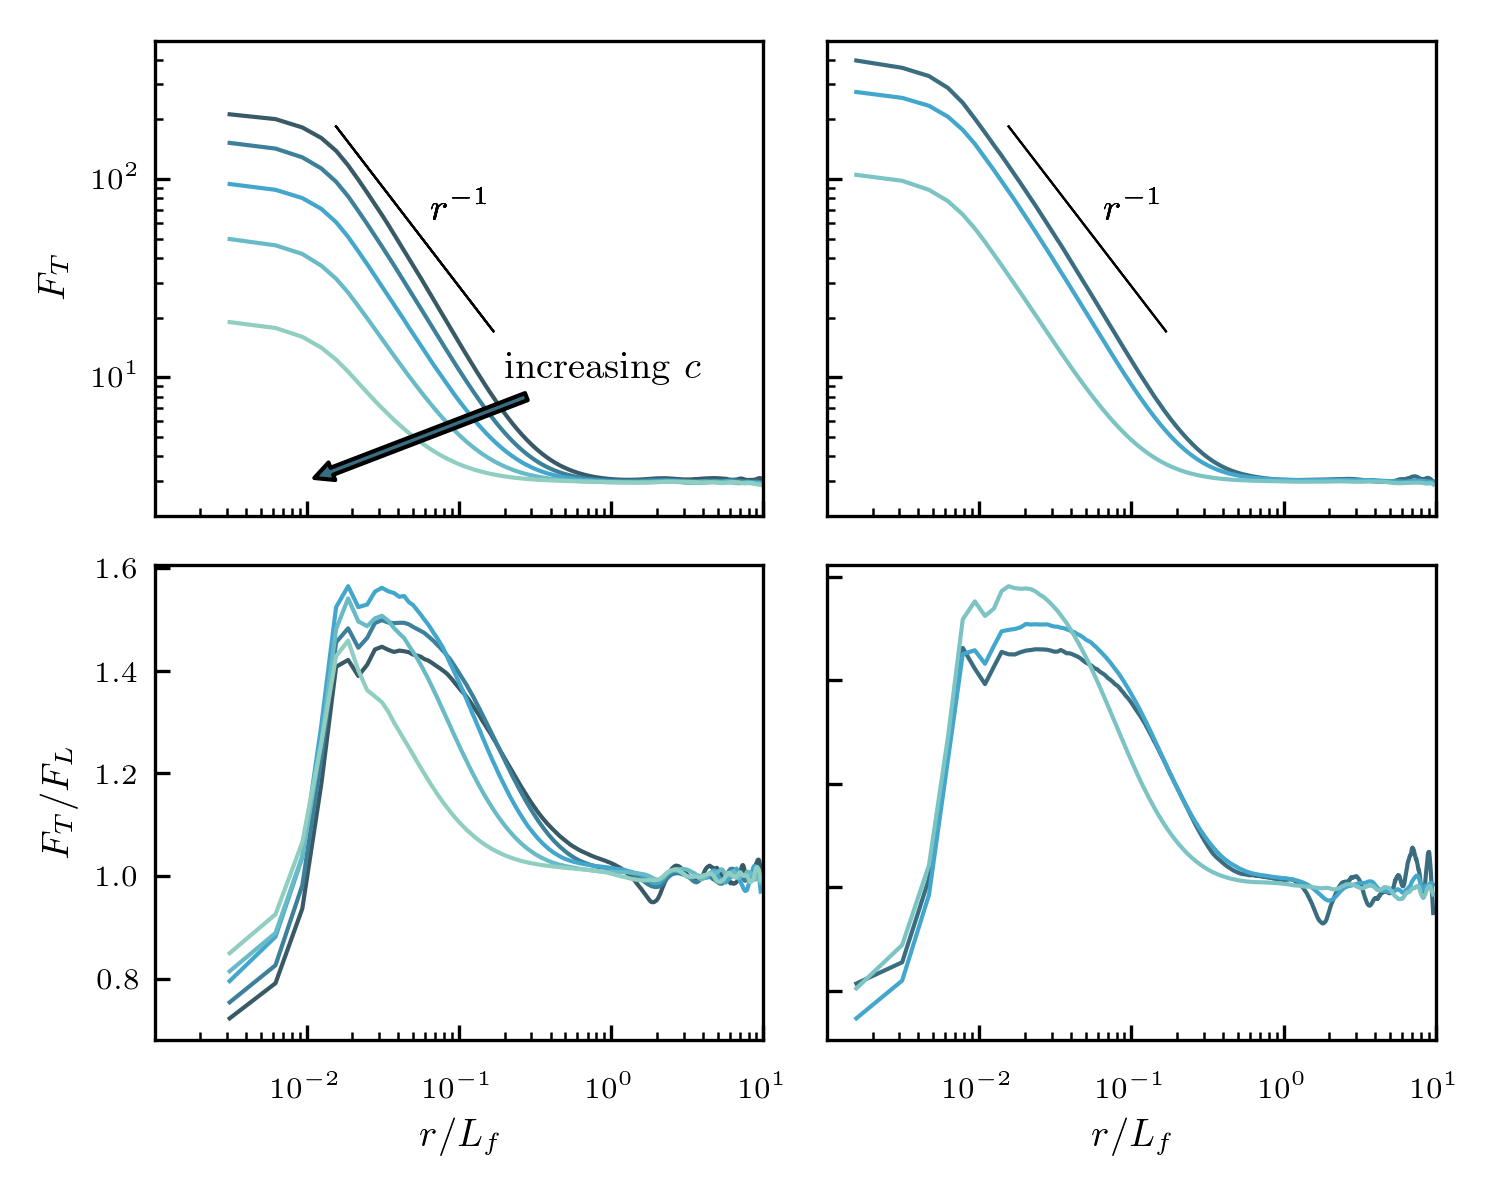
\includegraphics[width=12cm]{../Pyfig/fig_flatness}}
\caption{ Flatness of the longitudinal and transverse increments for
$c = 10$ and $n = 7680$. The straight continuous lines indicate the
$r^{-1}$-scaling and the straight dashed line the $r^{-3/2}$-scaling.
The inset shows the ratio $F_T/F_L$ and the corresponding value computed by the shock model, $F_T/F_L = 1.5$.  }
\label{fig_flatness}
\end{figure}

\begin{figure}
\centerline{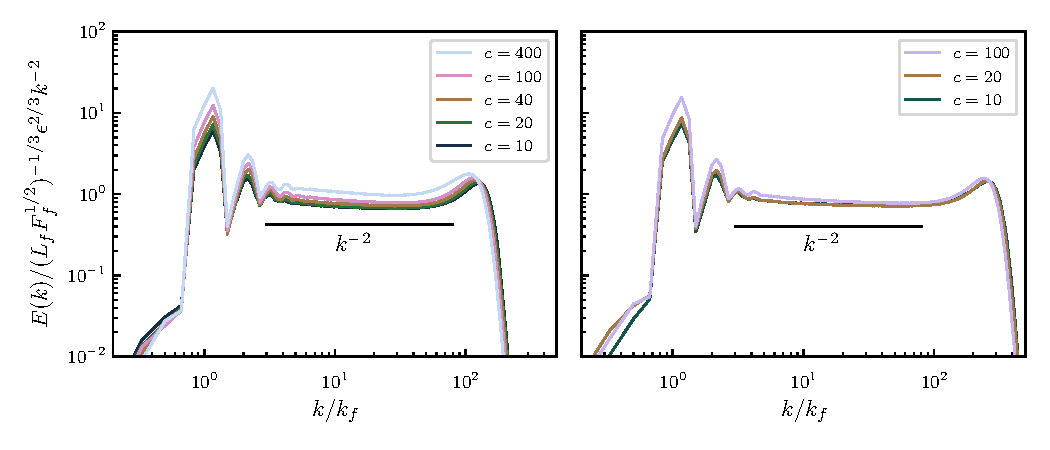
\includegraphics[width=11cm]{../Pyfig/fig_spectra}}
\caption{Compensated and normalised energy spectra
from runs with $ n = 7680 $: W4, W8 and W15.}
\label{fig_spectra_c40}
\end{figure}


We will now present the results for the structure functions. Substituting
(\ref{MeanDistance}) into (\ref{StrucFunc}) we find that the structure
functions are expected to scale as
\begin{equation} \label{StrucFunc2}
\meane{|\delta u |^p}  \sim \meane{(c|\delta h |)^p} \sim  (L_f F_f^{1/2})^{p/3-1}  \eps^{p/3}  r  \, .
\end{equation}
for separation distances that fulfill the condition $ \delta x \ll r \ll d $,
where $ \delta x $ is the shock width. The scaling (\ref{StrucFunc2}) is
expected to become better and better fulfilled with decreasing $ c $ (or
increasing $ F_f $), for two reasons. First, according to (\ref{MeanDistance})
$ d $ is increasing with $ F_f $, and the scaling range is therefore becoming
wider for decreasing $ c $, if $ \delta x $ or the resolution $ n $ is kept
constant. Second, according to (\ref{Strength}) the amplitude of the shocks
scales as $ (\eps d)^{1/3} $, which means that the shocks are becoming
increasingly strong for large $ d $ (small $ c $). Thus, the assumption that
the structure functions are totally dominated by increments where a shock is
crossed will be better fulfilled for small $ c $. This effect is expected to be
particularly important for lower order structure functions. The scaling
(\ref{StrucFunc2}) is also expected to become better and better fulfilled with
increased resolution $ n $, since $ \delta x $ is decreasing with increasing $
n $.

As expected, we have found that the displacement structure functions scale
exactly in the same way as the velocity structure functions, why we only plot
velocity structure functions. In figure~\ref{fig_StrucFunc} we see the
compensated and normalised second, fourth and sixth order longitudinal
structure functions from the five simulations with $ n = 3840 $ to the left and
the three simulations with $ n = 7860 $ to the right. At small separation, $ r
< \delta x $, the structure functions have the dependence $ \sim r^{p} $, which
is characteristic of a smooth velocity field, indicating that the shocks are
reasonably well resolved. There is a small bump around the shock width, $ r
\approx \delta x $, and at $ r > \delta x $, there is a range where the
compensated structure functions are flat, or almost flat. As expected, this
range is becoming broader for smaller $ c $ (or larger $ F_f $). The range is
also broader in the higher resolution runs to the right as compared to the
lower resolution simulations to the left. There is clearly a better collapse of
the curves for the sixth order structure functions compared to the second order
structure functions. This is not surprising, since the shock contribution to
the structure functions should become increasingly dominant with increasing
order. Plots of the transverse structure functions are very similar to the
plots of the longitudinal structure functions, with the difference that the
transverse structure functions are somewhat smoother at $ r \approx \delta x $.
In figure~\ref{fig_ratio} we see the ratio $ R_{p}(r) = \langle \mid \delta
u_L \mid ^{p} \rangle / \langle \mid \delta u_T \mid ^{p} \rangle$ for $ p=
2,3,4,5,6 $ from run W4, together with dotted straight lines, indicating the
values predicted by (\ref{Ratio}). As can be seen, there is a quite good
agreement with the predicted values in a limited range of separations, $ r >
\delta x $. Somewhat unexpectedly, the range in which there is a good agreement
becomes more narrow with increasing $ p $, an observation that we cannot
explain. It may also be noted that $ R_2 \rightarrow 3 $ in the limit of small
$ r $, which is the theoretical single point limit for an irrotational
isotropic field. In figure~\ref{fig_flatness} we se the flatness factor, $
F_T $, of the transverse structure functions at the top and the ratio, $
F_T/F_L $, at the bottom. The figures to the left show the results from the
five simulations with $ n = 3840 $ and the figures to the right show the
results from the three simulations with $ n = 7860 $. The flatness factor shows
increasingly large values for decreasing $ r $ with a dependence that is rather
close to but somewhat steeper than $ r^{-1} $. At small $ r $ the curves are
leveling out at very large values. For $ n = 7869 $ and $ c = 10 $ we see that
$ F_{T} \approx 400 $ at small $ r $. The degree to which the flatness factor
is increasing with decreasing scale is by some authors defined as the most
appropriate measure of spatial intermittency \cite[see for example][]{Frisch}.
If this measure is used, SW wave turbulence is, indeed, extremely intermittent.
In the two figures at the bottom we see that $ F_{T}/F_{L} \approx 1.5 $ in a
limited range of separations, $ r > \delta x $, which is becoming somewhat
broader as $ c $ is increasing and is also somewhat broader in the higher
resolution runs shown to the right as compared to the lower resolution runs
shown to the left. This is in accordance with the shock model predictions
(\ref{FL}) and (\ref{FT}).

Finally, we present energy spectra. As expected, we found that APE and KE
spectra were almost indistinguishable from each other, why we only plot the
total spectra. In figure~\ref{fig_spectra_c40} we see the compensated and
normalised energy spectra from the three highest resolution runs. The
compensated spectra are almost flat in a broad range. In the high wave number
end the compensated spectra show a `bottleneck', which we interpret as a
signature of the shocks, and at the very highest wave numbers the magnitude of
the spectra is strongly decreasing, indicating that the shocks are reasonably
well resolved. The $ k^{-2} $-dependence and the associated scaling predicted
by (\ref{Spectra}) are very well satisfied in a limited range of high wave
numbers close to the bottleneck. At smaller wave number the spectra are
becoming somewhat steeper than $ k^{-2} $ and the spectrum from the run with
largest $ c $ does not collapse perfectly onto the other two spectra.
